\documentclass[conference]{IEEEtran}
\usepackage{amsmath,amssymb,amsfonts}
\usepackage{graphicx}
\usepackage{textcomp}
\usepackage{xcolor}
\usepackage{braket}
\usepackage{caption}
\usepackage{subcaption}
\usepackage{float}
\usepackage{url} 

\title{Quantum Computation and Nonlinear Oscillators: Classical and Quantum Dynamics of a Duffing Oscillator and Schr\"odinger Cat States}

\author{Nilay D. Shenai}

\begin{document}

\maketitle

\begin{abstract}
This paper investigates the classical and quantum dynamics of nonlinear oscillators, specifically the Duffing oscillator model. We explore the evolution of quantum states relevant to quantum computation and quantum sensing, such as Schr\"odinger cat states, using numerical simulations and visualization tools. We model nonlinear effects via an $x^4$ (quartic) potential term and study their impact on quantum state evolution, expectation values, and Wigner functions.
\end{abstract}

\begin{IEEEkeywords}
Quantum computation, nonlinear oscillator, Duffing oscillator, Schr\"odinger cat state, Wigner function, coherent state
\end{IEEEkeywords}

\section{Introduction}
Quantum computation leverages superposition and entanglement to perform tasks beyond classical capabilities. Nonlinear oscillators, such as the Duffing oscillator, are of interest in quantum technologies due to their rich dynamical behavior. This paper explores:
\begin{itemize}
    \item Classical dynamics of the Duffing oscillator
    \item Quantum evolution under nonlinear Hamiltonians
    \item Behavior of coherent and Schr\"odinger cat states
    \item Visualization using Wigner functions
\end{itemize}

\section{Theory}
\subsection{Classical Duffing Oscillator}
The classical Duffing equation is:
\begin{equation}
    \frac{d^2x}{dt^2} + \delta \frac{dx}{dt} + \alpha x + \beta x^3 = 0
\end{equation}
where $\delta$ is damping, $\alpha$ linear stiffness, and $\beta$ nonlinear stiffness.

\subsection{Quantum Hamiltonian}
In the quantum case, we use the Hamiltonian:
\begin{equation}
    \hat{H} = \frac{\hat{p}^2}{2} + \frac{1}{2} \hat{x}^2 + \gamma \hat{x}^4
\end{equation}
with canonical commutation relation $[\hat{x}, \hat{p}] = i\hbar$.

\subsection{Cat States}
A Schr\"odinger cat state is a superposition of coherent states:
\begin{equation}
    \ket{\text{cat}} \propto \ket{+\alpha} + e^{i\phi}\ket{-\alpha}
\end{equation}
Cat states are used in quantum error correction and sensing.

\subsection{Wigner Function}
The Wigner function $W(x, p)$ is a quasi-probability distribution used to visualize quantum states in phase space.

\section{Methodology}
\begin{itemize}
    \item Classical dynamics: solved using \texttt{scipy.integrate.odeint}
    \item Quantum evolution: simulated using \texttt{qutip.mesolve}
    \item Observables: $\langle \hat{x}(t) \rangle$ and $\langle \hat{p}(t) \rangle$
    \item Wigner functions: visualized using \texttt{qutip.wigner}
\end{itemize}

\section{Results}
\subsection{Classical Duffing Oscillator}
Nonlinear oscillations and bifurcations were observed under varying parameters.

\begin{figure}[H]
    \centering
    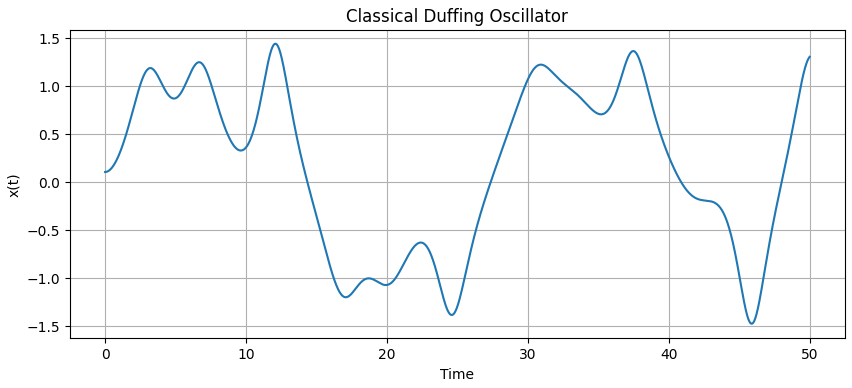
\includegraphics[width=0.9\linewidth]{duffing.png}
    \caption{Trajectory of the classical Duffing oscillator showing nonlinear behavior.}
    \label{fig:duffing_classical}
\end{figure}

\subsection{Quantum Coherent State}
\begin{itemize}
    \item Nearly harmonic oscillations
    \item Nonlinearity introduces slight distortions over time
\end{itemize}

\begin{figure}[H]
    \centering
    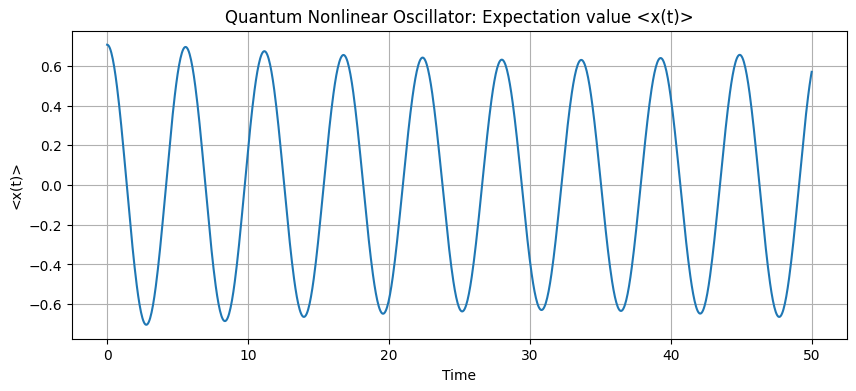
\includegraphics[width=0.9\linewidth]{coh.png}
    \caption{Quantum evolution of a coherent state: expectation value $\langle x(t) \rangle$.}
    \label{fig:coherent_xt}
\end{figure}

\subsection{Quantum Cat States}
\begin{itemize}
    \item Symmetric cat state ($\phi=0$) shows $\langle x(t) \rangle \approx 0$
    \item Asymmetric cat ($\phi \neq 0$) shows oscillatory $\langle x(t) \rangle$
\end{itemize}

\begin{figure}[H]
    \centering
    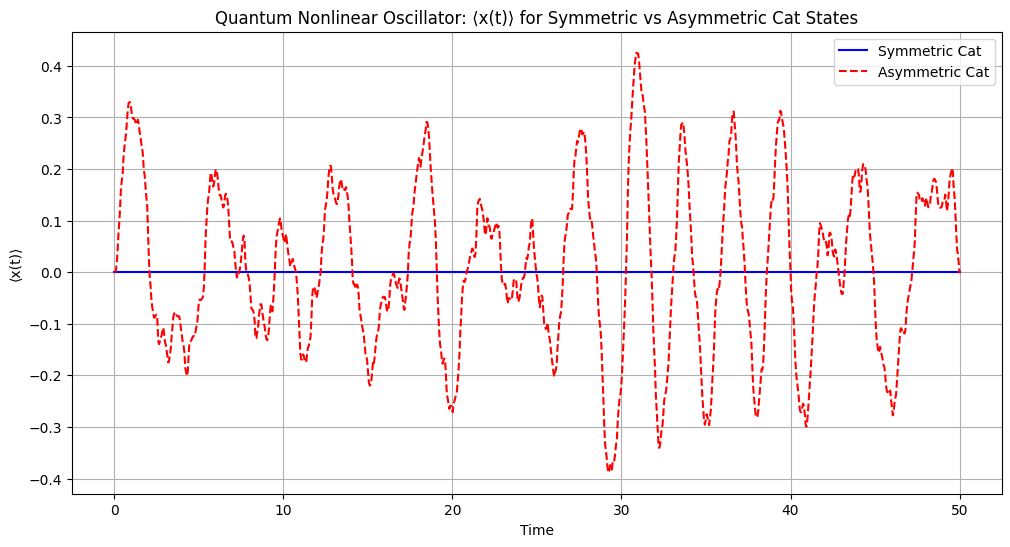
\includegraphics[width=0.9\linewidth]{3.png}
    \caption{Time evolution of $\langle x(t) \rangle$ for a symmetric Schr\"odinger cat state.}
    \label{fig:cat_xt}
\end{figure}

\subsection{Wigner Functions}
The Wigner function offers a phase-space representation of quantum states, revealing both classical and nonclassical features. For a coherent state, the Wigner function appears as a Gaussian-shaped distribution centered around its classical position.

\begin{figure}[H]
    \centering
    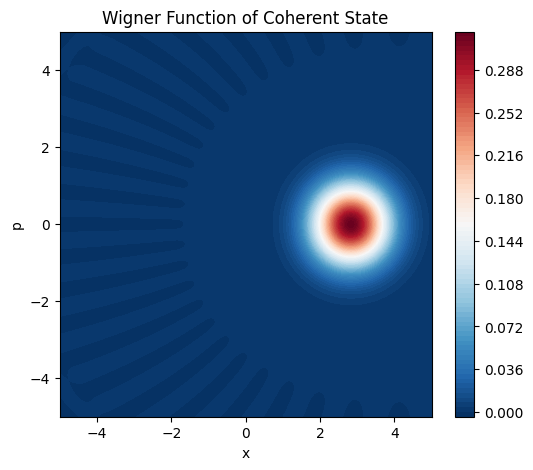
\includegraphics[width=0.9\linewidth]{4.png}
    \caption{Wigner function of a coherent state, showing a Gaussian distribution in phase space.}
    \label{fig:wigner_coherent}
\end{figure}

In contrast, the Wigner function of a Schr\"odinger cat state shows interference fringes between the two coherent components. These fringes are a signature of quantum coherence and are sensitive to decoherence mechanisms.

\begin{figure}[H]
    \centering
    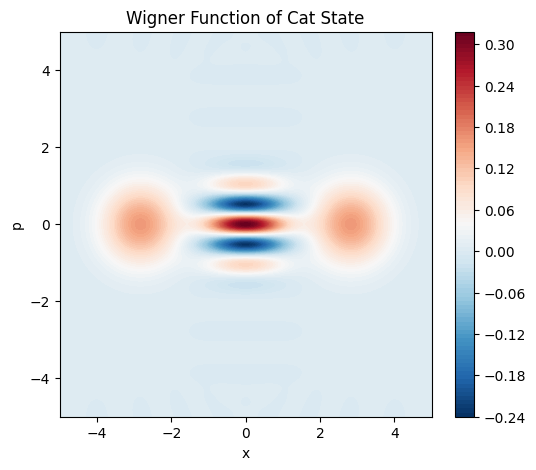
\includegraphics[width=0.9\linewidth]{5.png}
    \caption{Wigner function of a cat state, illustrating quantum interference fringes between two coherent peaks.}
    \label{fig:wigner_cat}
\end{figure}

\section{Discussion}
Our simulations validate several theoretical expectations:
\begin{itemize}
    \item The expectation value $\langle x(t) \rangle$ remains near zero for symmetric Schr\"odinger cat states due to destructive interference.
    \item Asymmetry in the cat state introduces measurable oscillations in $\langle x(t) \rangle$, reflecting its broken parity symmetry.
    \item Wigner functions prove highly effective in visualizing quantum features: coherent states exhibit classical-like Gaussian distributions, while cat states display clear interference fringes that signify quantum coherence.
\end{itemize}

These features are not only of theoretical interest but also relevant for quantum error correction and sensing protocols that exploit nonclassical states for enhanced performance.

\section{Conclusion}
We successfully simulated and analyzed the dynamics of classical and quantum Duffing oscillators. Nonlinearity plays a critical role in quantum evolution, especially in macroscopic superposition states. This work highlights how computational tools can elucidate deep quantum behaviors with practical relevance.

\begin{thebibliography}{00}
\bibitem{nielsen} M. A. Nielsen and I. L. Chuang, \textit{Quantum Computation and Quantum Information}, Cambridge University Press.
\bibitem{walls} D. F. Walls and G. J. Milburn, \textit{Quantum Optics}, Springer.
\bibitem{devoret} M. Devoret and R. Schoelkopf, "Superconducting Circuits for Quantum Information," \textit{Science}, vol. 304, pp.  772--777, 2004.
\bibitem{qutip} QuTiP Documentation, \url{https://qutip.org/}
\end{thebibliography}

\end{document}
